\documentclass{article}
\usepackage{geometry}
\geometry{
    a4paper,
    left=30mm,
    right=30mm,
    top=20mm,
    bottom=20mm
}


\usepackage{blindtext}
\usepackage{graphicx}
\usepackage{wrapfig}
% \usepackage{figure}

\graphicspath{ {./media/} }
\usepackage[square,numbers]{natbib}
\usepackage[nottoc]{tocbibind}
\usepackage{booktabs}
\usepackage{multirow}



\usepackage{tikz}
\usepackage{listings}
\usepackage{setspace}
\definecolor{Code}{rgb}{0,0,0}
\definecolor{Decorators}{rgb}{0.5,0.5,0.5}
\definecolor{Numbers}{rgb}{0.5,0,0}
\definecolor{MatchingBrackets}{rgb}{0.25,0.5,0.5}
\definecolor{Keywords}{rgb}{0,0,1}
\definecolor{self}{rgb}{0,0,0}
\definecolor{Strings}{rgb}{0,0.63,0}
\definecolor{Comments}{rgb}{0,0.63,1}
\definecolor{Backquotes}{rgb}{0,0,0}
\definecolor{Classname}{rgb}{0,0,0}
\definecolor{FunctionName}{rgb}{0,0,0}
\definecolor{Operators}{rgb}{0,0,0}
\definecolor{Background}{rgb}{0.98,0.98,0.98}
\lstdefinelanguage{Python}{
	numbers=left,
	numberstyle=\footnotesize,
	numbersep=1em,
	xleftmargin=1em,
	framextopmargin=2em,
	framexbottommargin=2em,
	showspaces=false,
	showtabs=false,
	showstringspaces=false,
	frame=l,
	tabsize=4,
	% Basic
	basicstyle=\ttfamily\small\setstretch{1},
	backgroundcolor=\color{Background},
	% Comments
	commentstyle=\color{Comments}\slshape,
	% Strings
	stringstyle=\color{Strings},
	morecomment=[s][\color{Strings}]{"""}{"""},
	morecomment=[s][\color{Strings}]{'''}{'''},
	% keywords
	morekeywords={import,from,class,def,for,while,if,is,in,elif,else,not,and,or,print,break,continue,return,True,False,None,access,as,,del,except,exec,finally,global,import,lambda,pass,print,raise,try,assert},
	keywordstyle={\color{Keywords}\bfseries},
	% additional keywords
	morekeywords={[2]@invariant,pylab,numpy,np,scipy},
	keywordstyle={[2]\color{Decorators}\slshape},
	emph={self},
	emphstyle={\color{self}\slshape},
	%
}

\title{\textbf{Proposal for bachelor thesis}\\
Exploration of the influence of graph parameters on the generalization error of Graph Neural Networks}

\author{Author: Wensheng Zhang}

\date{\today}

\begin{document} 

\maketitle

\tableofcontents


\begin{abstract}
The goal of this bachelor thesis is to understand empirically how graph parameters/characteristics influence the generalization error of Graph Neural Networks (GNNs).
\end{abstract}


\section{Introduction}

What is graph parameters? Graph parameters are the properties of the graph, which can be calculated from the graph. For example, the average degree of the graph, the average shortest path of the graph, the average number of coloring in the 1-WL algorithm, etc. In the early experiment, the graph parameters are calculated as the average degree and the average shortest path of the graphs.
\\
In the another hand, the generalization error is a measure of how well the model generalizes to unseen data. In the experiment, the generalization error is calculated as the difference between the training accuracy and the test accuracy.
\\
Why is it important to understand the influence of graph parameters on the generalization error of GNNs? The understanding of the influence of graph parameters on the generalization error of GNNs can help us to understand the behavior of GNNs. For example, if we know that the average degree of the graph has a significant influence on the generalization error of GNNs, we can design GNNs that are more robust to the average degree of the graph.



\section{Setup in the early experiment}
In following, I will descripe training framework, datasets and models for the setup of the experiment.

\subsection{Training Framework}
The training framework is based on PyTorch Geometric~\cite{fey2019fast}. PyTorch Geometric is a library for deep learning on graphs and other irregular structures. It consists of various methods and utilities to ease the implementation of GNNs.

\subsection{Datasets}
The dataset in the experiment is TUDataset~\cite{morris_tudataset_2020}. TUDataset is often used for the GNN evaluation. It consists data across different domains, including small molecules, bioinformatics, social networks and synthetic. Since the size of some datasets are quiet small (under 500 data points/graphs), I use 10-fold cross validation in the training process, in order to fully utilize the data. A dataset is splited into 1:1:8, inwhich one of the folds is treated as test dataset and another is treated as validation dataset. The rest of the folds are used for training. 

\subsection{Models}
In the early experiment, I have used GCN layer~\cite{kipf2017semisupervised} and GAT layer~\cite{velickovic2020pointer}. To prevent overfitting, dropout is used in the model. Relu is used as activation function. In the Appendix, I have provided the code of example models.


\section{Experiment}
% 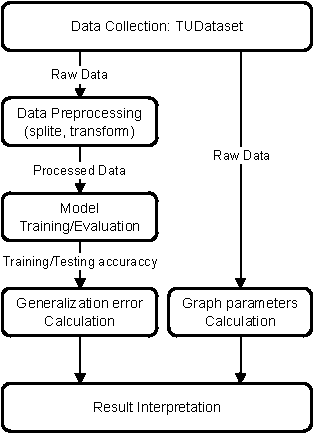
\includegraphics{experiment_procedure.pdf}


\begin{figure}[h]
    \centering
    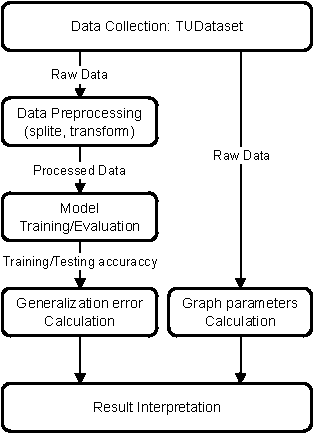
\includegraphics[width=0.5\textwidth]{experiment_procedure.pdf}
    \caption{A illutration of experiment Procedure}
    \label{fig:experiment}
\end{figure}

The experiment consists in three parts: 1. Train the models from datasets and evaluate the models to calculate the generalization error. 2. calculate the parameters of the graphs from the dataset. 3. Analyze the influence of the graph parameters on the generalization error of the GNNs. (See Figure~\ref{fig:experiment})


\subsection{Experimental details in the early stage}
I use Adam optimizer with learning rate 0.01. The batch size is set to 64. The hidden dimension of the GNN layer is set to 64. The number of epochs is set to 200. To prevent overfitting and to save time, the early stopping is used with patience 20. The loss function is set to CrossEntropyLoss. 

\section{Results}

Here I take seven datasets from TUDataset as examples. The calculated parameters are shown in Table~\ref{tab:parameter}. The generalization error of the models are shown in Table~\ref{tab:error}. 

\begin{table}[h!]
    \centering
    \begin{tabular}{@{}lll@{}}
    \toprule
    \multicolumn{1}{c}{\multirow{2}{*}{Dataset}} & \multicolumn{2}{c}{Parameter}                                            \\ \cmidrule(l){2-3} 
    \multicolumn{1}{c}{}                         & \multicolumn{1}{c}{Ave. degree} & \multicolumn{1}{c}{Ave. shortest path} \\ \midrule
    Mutagenicity                                 & 2.0379         & 4.4825                     \\
    NCI1                                         & 2.1550         & 5.4697                     \\
    COIL-RAG                                     & 1.8277         & 1.0606                     \\
    Letter-high                                  & 1.8896         & 1.5173                     \\
    DD                                           & 4.9790         & 7.9700                     \\
    PTOTEIN\_full                                & 3.7346         & 4.7123                     \\
    COLORS-3                                     & 2.9288         & 2.0945                     \\ \bottomrule
    \end{tabular}
    \caption{The calculated parameters from a set of datasets}
    \label{tab:parameter}
\end{table}

\begin{table}[h!]
    \centering
    \begin{tabular}{@{}lll@{}}
    \toprule
    Dataset        & Ave. generalization error & Standard Deviation   \\ \midrule
    Mutagenicity   & 0.0268      & 0.02335 \\
    NCI1           & 0.0138      & 0.02649 \\
    COIL-RAG       & 0.0450      & 0.01378 \\
    Letter-high    & 0.0403      & 0.04342 \\
    DD             & 0.0524      & 0.05849 \\
    PROTEINS\_full & 0.0189      & 0.05032 \\
    COLORS-3       & 0.0076      & 0.01428 \\ \bottomrule
    \end{tabular}
    \caption{The calculated generalization error from a set of datasets}
    \label{tab:error}
\end{table}

Then I plot the generalization error against the graph parameters. The result is shown in Figure~\ref{fig:scatter}.

\begin{figure}[h!]
    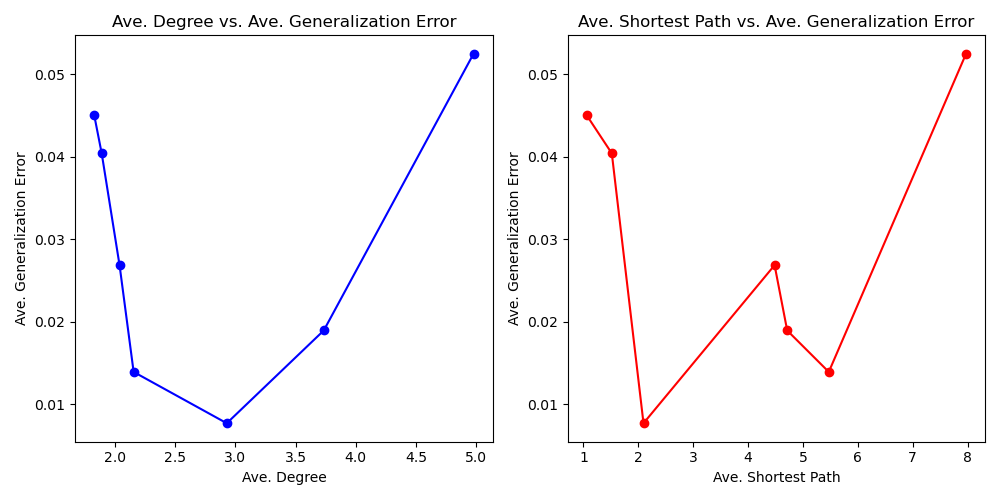
\includegraphics[width=\textwidth]{final_results.png}
    \caption{The generalization error against the graph parameters}
    \label{fig:scatter}
\end{figure}

\section{In the further work}
In the future, I plan to explore different GNN layers and datasets to evaluate the consistency of the results. Additionally, I will consider experimenting with various graph parameters. In \cite{gera2018annotated}, the authors have proposed a set of graph parameters that can be used to characterize the graph. I will use these parameters in the future work.

\newpage

\bibliographystyle{abbrvnat} % or another style like unsrt, alpha, etc.
\bibliography{bibliography} % refers to example.bib

% All reduce Graphs
\newpage 

\section{Appendix} 
 
\subsection*{Example of GCN model}

\begin{lstlisting}[language=Python]
import torch
from torch import nn
import torch.nn.functional as F
from torch_geometric.nn import GCNConv
from torch_geometric.nn import global_mean_pool


class GCN(torch.nn.Module):
    def __init__(self, in_channels, hidden_channels, out_channels):
        super().__init__()
        self.conv1 = GCNConv(in_channels, hidden_channels)
        self.conv2 = GCNConv(hidden_channels, hidden_channels)
        self.conv3 = GCNConv(hidden_channels, hidden_channels)
        self.conv4 = GCNConv(hidden_channels, hidden_channels)
        self.fc1 = nn.Linear(hidden_channels, hidden_channels)
        self.fc2 = nn.Linear(hidden_channels, out_channels)


    def forward(self, x, edge_index, batch, edge_weight=None):
        x = self.conv1(x, edge_index, edge_weight).relu()
        x = self.conv2(x, edge_index, edge_weight).relu()
        x = self.conv3(x, edge_index, edge_weight).relu()
        x = self.conv4(x, edge_index, edge_weight).relu()
        x = global_mean_pool(x, batch)
        x = self.fc1(x).relu()
        x = F.dropout(x, p=0.5, training=self.training)
        x = self.fc2(x)
        return x
    
    def reset_parameters(self):
        for (_, module) in self._modules.items():
            module.reset_parameters()

\end{lstlisting}

\end{document}